%%%%%%%%%%%%%%%
%
%	MAT101 Øving 1 Løsning
%
%	Oskar L. F. Leirvåg
%
%

\documentclass[norsk, a4paper, 12pt,]{article}
\usepackage[norsk]{babel}
\usepackage[utf8]{inputenc}
\usepackage[utf8]{inputenc}
\usepackage[T1]{fontenc}
\usepackage{url}
\def\UrlBreaks{\do\/\do-}
\usepackage{fixltx2e}
\usepackage{graphicx}
\usepackage{xcolor}
\usepackage{caption}
\usepackage{float}
\usepackage{wrapfig}
\usepackage{amssymb}
\usepackage[colorinlistoftodos,prependcaption,textsize=tiny]{todonotes}
\usepackage{soul}
\usepackage{textcomp}
\usepackage{marvosym}
\usepackage[integrals]{wasysym}
\usepackage{latexsym}
\usepackage{amssymb}
\usepackage{hyperref}
\tolerance=1000
\usepackage{amsmath}
\usepackage{hyperref}
\usepackage{setspace}
\onehalfspacing
\usepackage[raggedright,bf,sf]{titlesec}
\usepackage{fullpage}
\usepackage{xcolor}
\usepackage{listings}
\lstset{basicstyle=\ttfamily,
  showstringspaces=false,
  commentstyle=\color{gray},
  keywordstyle=\color{blue}
}

%Margins
\usepackage{geometry}
\geometry{a4paper, margin=1in}

%Definitions
\def\mathUnderline#1{\underline{\underline{#1}}}

\begin{document}
\begin{titlepage}


\newcommand{\HRule}{\rule{\linewidth}{0.5mm}} % Defines a new command for the horizontal lines, change thickness here

\center % Center everything on the page

%----------------------------------------------------------------------------------------
%	HEADING SECTIONS
%----------------------------------------------------------------------------------------

\textsc{\LARGE Universitetet i Bergen}\\[1.5cm] % Name of your university/college
\textsc{\Large DAT103}\\[0.5cm] % Major heading such as course name
\textsc{\large Datamaskiner og operativsystem}\\[0.5cm] % Minor heading such as course title

%----------------------------------------------------------------------------------------
%	TITLE SECTION
%----------------------------------------------------------------------------------------

\HRule \\[0.4cm]
{ \huge \bfseries Øvelse 3: Assembly}\\[0.4cm] % Title of your document
\HRule \\[1.5cm]

%----------------------------------------------------------------------------------------
%----------------------------------------------------------------------------------------
%	AUTHOR SECTION
%----------------------------------------------------------------------------------------
\Large \emph{Author:}\\
Oskar L. F. Leirvåg\\Stud nr: 570984
\\[2cm] % Your name
%----------------------------------------------------------------------------------------
\centerline{
\includegraphics[scale=0.15]{figures/canvas}} % Include a department/university logo - this will require the graphicx package
%----------------------------------------------------------------------------------------
%	DATE SECTION
%----------------------------------------------------------------------------------------

{\large \today}\\[3cm] % Date, change the \today to a set date if you want to be precise

%----------------------------------------------------------------------------------------
%	LOGO SECTION
%----------------------------------------------------------------------------------------

\vfill % Fill the rest of the page with whitespace

\end{titlepage}

% TASK ONE
% % % % % % % % % % % % % % % % %

\section*{Forklaring av kjøreflagg:}
\subsection*{Kompiler:}

Alle programmene kompileses med \begin{verbatim}
nasm –f elf –F dwarf –g <filnavn>.asm \end{verbatim}
som gir en ``<filnavn>.o fil.''

\begin{itemize}
  \item [-f] bestemmer format som vi her setter til elf som er et
  ``Executable and Linkable Format''. Dette er et format som prøver å
  virke på flest mulig prosessor-arkitekturer.

  \item [-F] med Debug-format til dwarf, som er ment å fungere best mulig sammen med elf
  formatet, og som åpner for et debuggable format for bruk i GDB.

  \item [-g] Tvinger NASM til å produsere debug informasjon
\end{itemize}


\subsection*{Link:}
For å bruke denne binærfilen må vi igjen gjøre den kjørbar med ``ld'' kommandoen. Da brukte jeg de gitte parametere:  \begin{verbatim}
  ld –m elf_i386 –o <nyFil> <filnavn>.o \end{verbatim}

\begin{itemize}
  \item [-m] bestemmer en emulering av i386 systemet slik at prosessor-
  arkitekturen blir satt til 32bit.

  \item [-o] bestemmer navnet på output filen etterfulgt av en filnavn uten
  suffix. Denne blir da kjørbar med ./<filnavn>
\end{itemize}
\newpage
\subsection*{Debug:}
For nå å kjøre filen kan den enkelt kjøres med ./<filnavn> men dette vil bare
kjøre den rett i systemet. Dersom vi ønsker en de-bugger må vi åpne den i GDB.
Dette kan gjøres med kommando, som gir os et 31 år
gammel UI som er absolutt horribel, bugger hele tiden og kan gi problemer med
kjøring.
\begin{verbatim}
  gdb –tui <nyFilNavn>
\end{verbatim}

\begin{itemize}
  \item [-tui] er her nødvendig for å gi en grafisk fremmstilling, av koden i et
  lite vindu. Her kan vi og bruke "layout regs". Til å åpne en grafisk
  fremmstilling av registry.

  \item [b] vil sette et breakpoint på bestemt linje.

  \item [r] starter programmet og eksekverer fremm til neste breakpoint.

  \item [si] er step funksjon (bedre enn s) og vil bare ta et enkelt steg videre i koden
  som highlightes i konsoll/vindu dersom det er startet med \-tui.
\end{itemize}

% DEL 2
% % % % % % % % % % %
\section*{Eksempelkjøring:}
\subsection{Script:}
\begin{verbatim}
Script started on Wed 25 Oct 2017 17:48:04 CEST
raknoel@Poseidon:~$ ls
hello  loop  totall  typescript
raknoel@Poseidon:~$ cd hello/
raknoel@Poseidon:~/hello$ ls
hello  hello.asm  hello.o  typescript
raknoel@Poseidon:~/hello$ ./hello
Hello World!
raknoel@Poseidon:~/hello$ cd ..
raknoel@Poseidon:~$ cd loop/
raknoel@Poseidon:~/loop$ ./loop
00
raknoel@Poseidon:~/loop$ cd ..
raknoel@Poseidon:~$ cd totall/
raknoel@Poseidon:~/totall$ ls
toTall  toTall.asm  toTall.o
raknoel@Poseidon:~/totall$ ./toTall
Skriv to ensifrede tall skilt med mellomrom.
Summen av tallene maa vaere mindre enn 10.
2 2

04
raknoel@Poseidon:~/totall$
raknoel@Poseidon:~/totall$ ./toTall
Skriv to ensifrede tall skilt med mellomrom.
Summen av tallene maa vaere mindre enn 10.
4 3

07
raknoel@Poseidon:~/totall$
raknoel@Poseidon:~/totall$ ./toTall
Skriv to ensifrede tall skilt med mellomrom.
Summen av tallene maa vaere mindre enn 10.
1 1

02
raknoel@Poseidon:~/totall$
raknoel@Poseidon:~/totall$ ./toTall
Skriv to ensifrede tall skilt med mellomrom.
Summen av tallene maa vaere mindre enn 10.
9   9

18
raknoel@Poseidon:~/totall$
raknoel@Poseidon:~/totall$ ./toTall
Skriv to ensifrede tall skilt med mellomrom.
Summen av tallene maa vaere mindre enn 10.
1 9

10
raknoel@Poseidon:~/totall$
\end{verbatim}

\subsection{Image?:}
\centerline{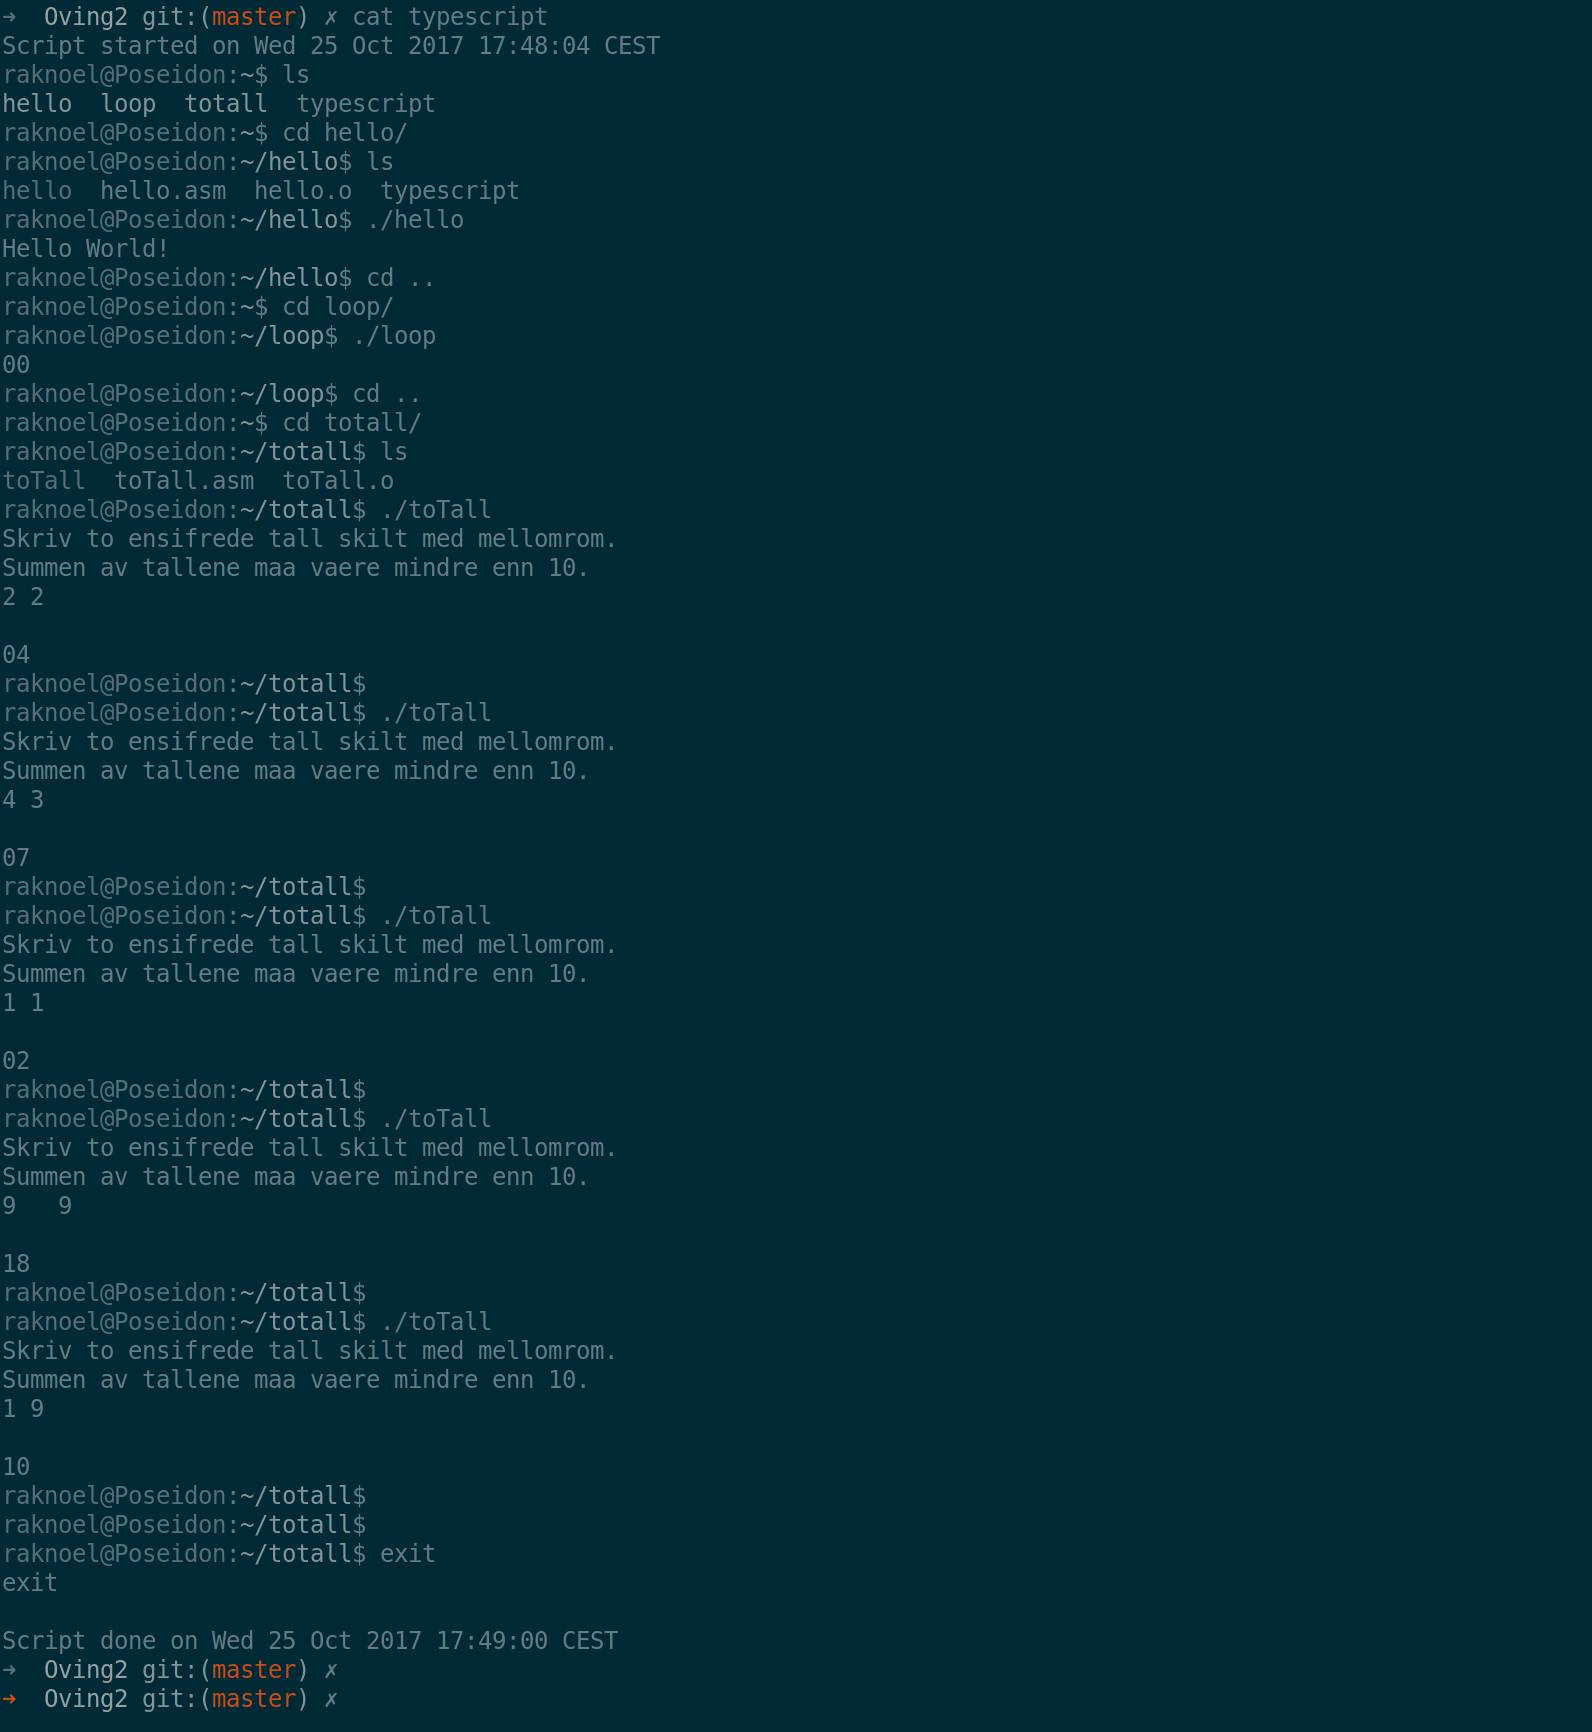
\includegraphics[scale=0.4]{figures/screenshot}}


\end{document}
